
Tjis manufactured solution originates in \textcite{john16} (book).
The stream function is given by
\[
\Phi(x,y) = 1000x^2(1-x)^4 y^3 (1-y)^2 = 1000 f(x)g(y)
\]
with 
\begin{eqnarray}
f(x)&=& x^2(1-x)^4 \nn\\
f'(x) 
&=& 2x (1-x)^4 - 4x^2 (1-x)^3 \nn\\
&=& [2x(1-x) -4x^2] (1-x)^3 \nn\\
&=& (2x-6x^2) (1-x)^3 \nn\\
&=& 2x(1-3x) (1-x)^3 \nn\\
f''(x) 
&=& 2(1-3x)(1-x)^3 -6x (1-x)^3 -6x(1-3x)(1-x)^2 \nn\\
&=& 2[ (1-3x)(1-x) -3x(1-x) -3x(1-3x)  ] (1-x)^2 \nn\\
&=& 2[ 1-4x+3x^2 -3x+3x^2 -3x+9x^2 ] (1-x)^2 \nn\\
&=& 2(1-10x+15x^2)(1-x)^2 \nn\\
f'''(x)
&=& 2[(-10+30x)(1-x)^2 -2 (1-10x+15x^2)(1-x)] \nn\\
&=& 2[-10+40x-30x^2  -2+20x-30x^2 ](1-x) \nn\\
&=& 2(-12+60x-60x^2 )(1-x) \nn\\
&=& 24 (-1+5x-5x^2 )(1-x) \nn\\
&=& 24(-1+5x-5x^2+x-5x^2+5x^3) \nn\\
&=& 24(-1+6x-10x^2+5x^3 ) \nn\\
\nn\\
g(y) &=& y^3(1-y)^2 \nn\\
g'(y) 
&=& 3y^2(1-y)^2 -2y^3 (1-y) \nn\\
&=& [3y^2(1-y) -2y^3] (1-y) \nn\\
&=& y^2 (3-3y-2y) (1-y) \nn\\
&=& y^2 (3-5y) (1-y) \nn\\
g''(y) 
&=& 2y (3-5y) (1-y) -5y^2  (1-y) -y^2 (3-5y)  \nn\\
&=& 2y(3-8y+5y^2) -5y^2 + 5y^3 - 3y^2 + 5y^3 \nn\\
&=& 6y -16y^2 + 10y^3 -8y^2 +10y^3 \nn\\
&=& 2y(3 -12y+10y^2) \nn\\
g'''(y) 
&=& 6 - 48y +60y^2 \nn
\end{eqnarray}

\begin{eqnarray}
u(x,y) 
&=& \partial_y \Phi 
= 1000 f(x) g'(y) = 1000 x^2(1-x)^4  y^2 (3-5y) (1-y) \\
v(x,y) &=& -\partial_x \Phi 
= -1000 f'(x) g(y)  = -1000 2x(1-3x) (1-x)^3  y^3(1-y)^2   \\
p(x,y) &=& \pi^2 [xy^3 \cos(2\pi x^2 y) - x^2y \sin(2\pi xy) ]+1/8
\end{eqnarray}

\begin{center}
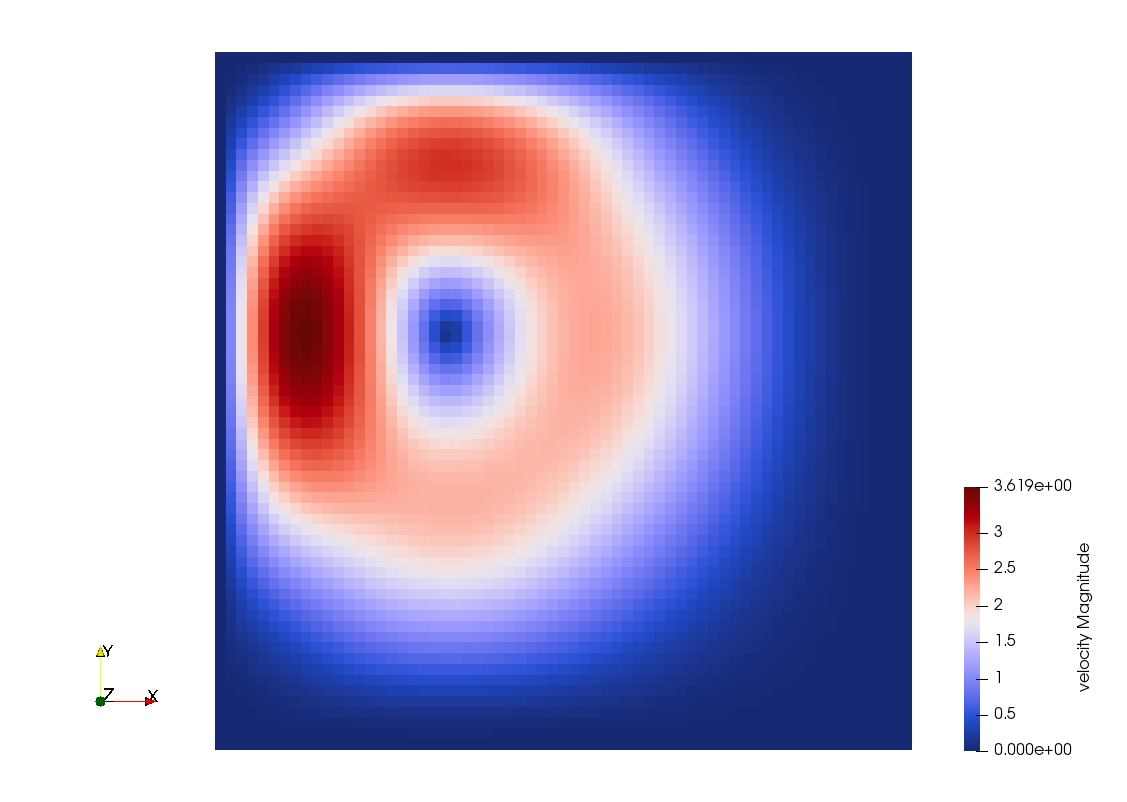
\includegraphics[width=5cm]{images/mms/mms_johnbook_vel}
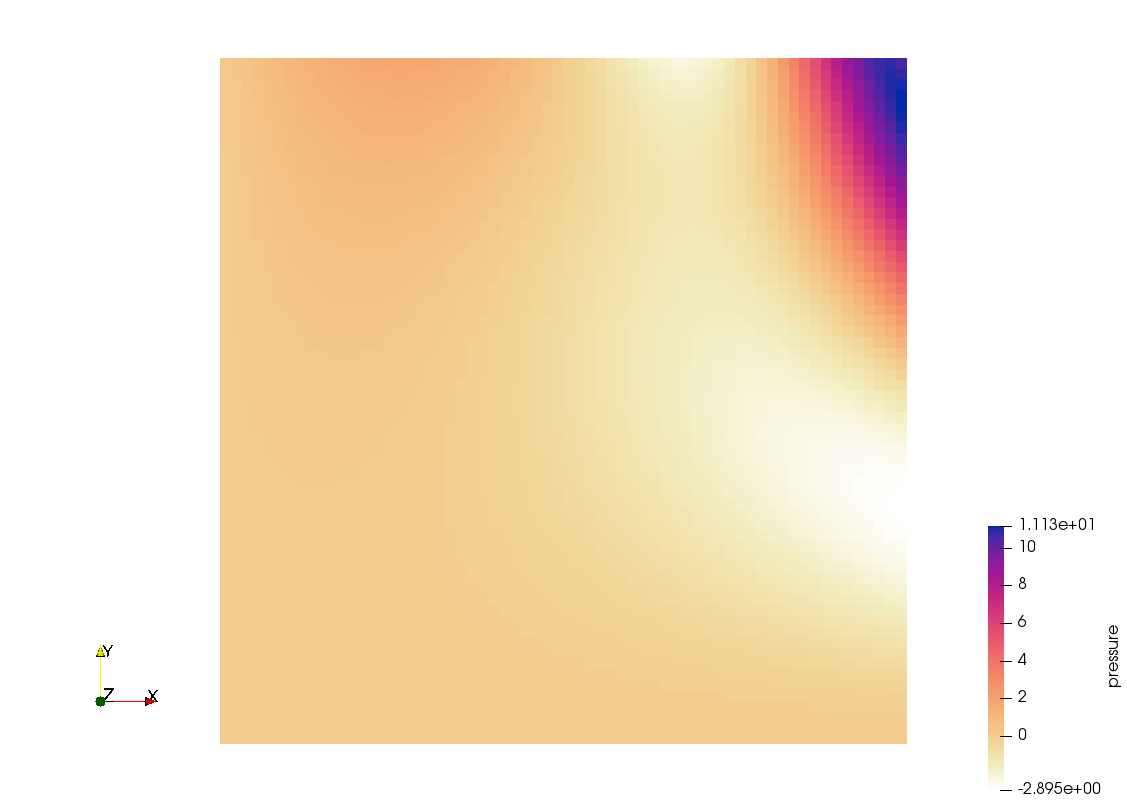
\includegraphics[width=5cm]{images/mms/mms_johnbook_press}
\end{center}


\begin{eqnarray}
\partial_x u (x,y)&=& 1000f'(x)g'(x)\nn\\
\partial_y u (x,y)&=& 1000f(x)g''(y) \nn\\
\partial_x v (x,y)&=& -1000f''(x)g(y) \nn\\
\partial_y v (x,y)&=& -1000f'(x)g'(y)\nn\\
\dot\varepsilon_{xx}(x,y) &=& 1000f'g' \nn\\
\dot\varepsilon_{yy}(x,y) &=& -1000f'g' \nn\\
\dot\varepsilon_{xy}(x,y) &=&  500( fg'' - f''g )\nn\\
\partial_x \dot\varepsilon_{xx} (x,y)&=& 1000f''g'\nn\\
\partial_x \dot\varepsilon_{xy} (x,y)&=& 500( f'g'' - f'''g )\nn\\
\partial_y \dot\varepsilon_{xy} (x,y)&=& 500( fg''' - f''g' )\nn\\
\partial_y \dot\varepsilon_{yy} (x,y)&=&  -1000f'g''\nn
\end{eqnarray}

Of course we have $\dot\varepsilon_{xx}+\dot\varepsilon_{yy}=0$.

\begin{eqnarray}
\frac{\partial p}{\partial x} (x,y)
&=& \pi^2 [ y^3 \cos(2\pi x^2 y) -4\pi x^2y^4  \sin(2\pi x^2 y) -2xy \sin(2\pi x y) -2 \pi x^2 y^2 \cos(2\pi x y)  ]\nn\\
\frac{\partial p}{\partial y} (x,y)
&=& \pi^2 [3xy^2 \cos(2\pi x^2 y) -2\pi x^3y^3\sin(2\pi x^2 y)
-x^2 \sin(2\pi x y) -2\pi x^3 y \cos(2\pi x y) ]
\nn
\end{eqnarray}


\begin{eqnarray}
\upnu_{rms}
&=&\sqrt{ \frac{1}{L_xL_y} \iint (u^2+v^2) dxdy   }  \nn\\
&=&\sqrt{  \int_0^1\int_0^1 u^2 \; dxdy  +  \int_0^1\int_0^1 v^2 \; dxdy } \nn\\
&=&1000\sqrt{  \int_0^1\int_0^1 (fg')^2\; dxdy  +  \int_0^1\int_0^1 (-f'g)^2 \; dxdy } \nn\\
&=&1000\sqrt{  
\underbrace{\int_0^1 f^2 dx }_{\frac{1}{6435}}
\underbrace{\int_0^1 g'^2 dy  }_{\frac{2}{315}}
+  
\underbrace{\int_0^1 f'^2 dx}_{\frac{2}{693}} 
\underbrace{\int_0^1 g^2 dy}_{\frac{1}{2310}} 
} \nn\\
&=& 1000 \sqrt{ \frac{1}{5\cdot 9 \cdot 13 \cdot 11} \frac{2}{5\cdot 9\cdot 7} + \frac{1}{9\cdot 11 \cdot 7} \frac{1}{5 \cdot 11 \cdot 3 \cdot 7}} \nn\\
&\simeq& 1.4953325891041323968540981
\end{eqnarray}


